\documentclass[a4paper]{article}
\usepackage[utf8]{inputenc}
\usepackage[margin=1.5in]{geometry}
\usepackage{datatool}

\usepackage[space]{grffile}

\usepackage{lscape}

\usepackage{wrapfig}
\usepackage{graphicx}
\usepackage{grffile}

\usepackage{rotating}

\title{Emergent Architecture Design}
\author{Joe Harrison \and Harm Griffioen \and Dereck Bridie \and Paul van der Knaap \and Natasa Radenovic}
\date{\today}

\begin{document}

\maketitle

\section{Introduction}
In this document we will go over the details of how the system is going to be built and how our group will design the software architecture of the connector part of our context project. 

\section{Design goals}
Throughout the project, the contributors will keep certain design goals in mind when creating code for our project.

\subsection{Availability}
Since a group is reliant on us to perform, it is important that they are able to receive new versions of our software when they need it. To achieve that, we will create tooling so that that group can download cutting-edge new releases. We will be able to incorporate feedback when they have requests.

\subsection{Extensibility}
Keeping in mind that the Tygron Engine is not final and may be changed by Tygron in the future, we will design our Connector in such a way that features can easily be added, removed or modified when the Tygron Engine changes.

Adding Tygron objects to our Environment is simple due to the way our Loaders work. To add percepts for the Agent, only a Loader has to be created and registered. 

\subsection{Performance}
The Connector should have low latency, so that agents can ask for environment information and be able to process this information without our Connector being the bottleneck. 

To achieve this, we have a separate thread that asynchronously requests environment data from the server so that the agent can perform without having to wait for these results.

\subsection{Code quality}
The Connector's code will be of high-quality, which means that code will be dynamically and statically tested. To check the quality of our code we will be using various tools which give indications of code quality. 

Our code repository is split up into multiple branches. One branch, \textbf{master}, is the main branch in which code will be stored that is working. Every change to the code in the master branch must be manually reviewed and approved by a majority of us before being allowed to be pulled to the master branch.

\textbf{CheckStyle} is a development tool that helps programmers write Java code that adheres to a coding standard. This will help us create code that has uniform code styling, keeping into account white space, method length, documentation, and so on.

\textbf{PMD} and \textbf{FindBugs} are source code analyzers which finds common programming flaws and reports them.

\textbf{JUnit} is a testing framework which allows programmers to write repeatable tests. In conjunction with \textbf{Cobertura}, this can be used to  check the percentage of code accessed by tests.

\textbf{Javadoc} will be used to generate documentation which will be used to describe code. %needs more

All of these tools will be run together using \textbf{Travis} and \textbf{Jenkins} Continuous Integration. These tools will automatically generate reports based on latest versions of code.

\noindent
\begin{sidewaysfigure}[ht]
\section{Class Diagram}
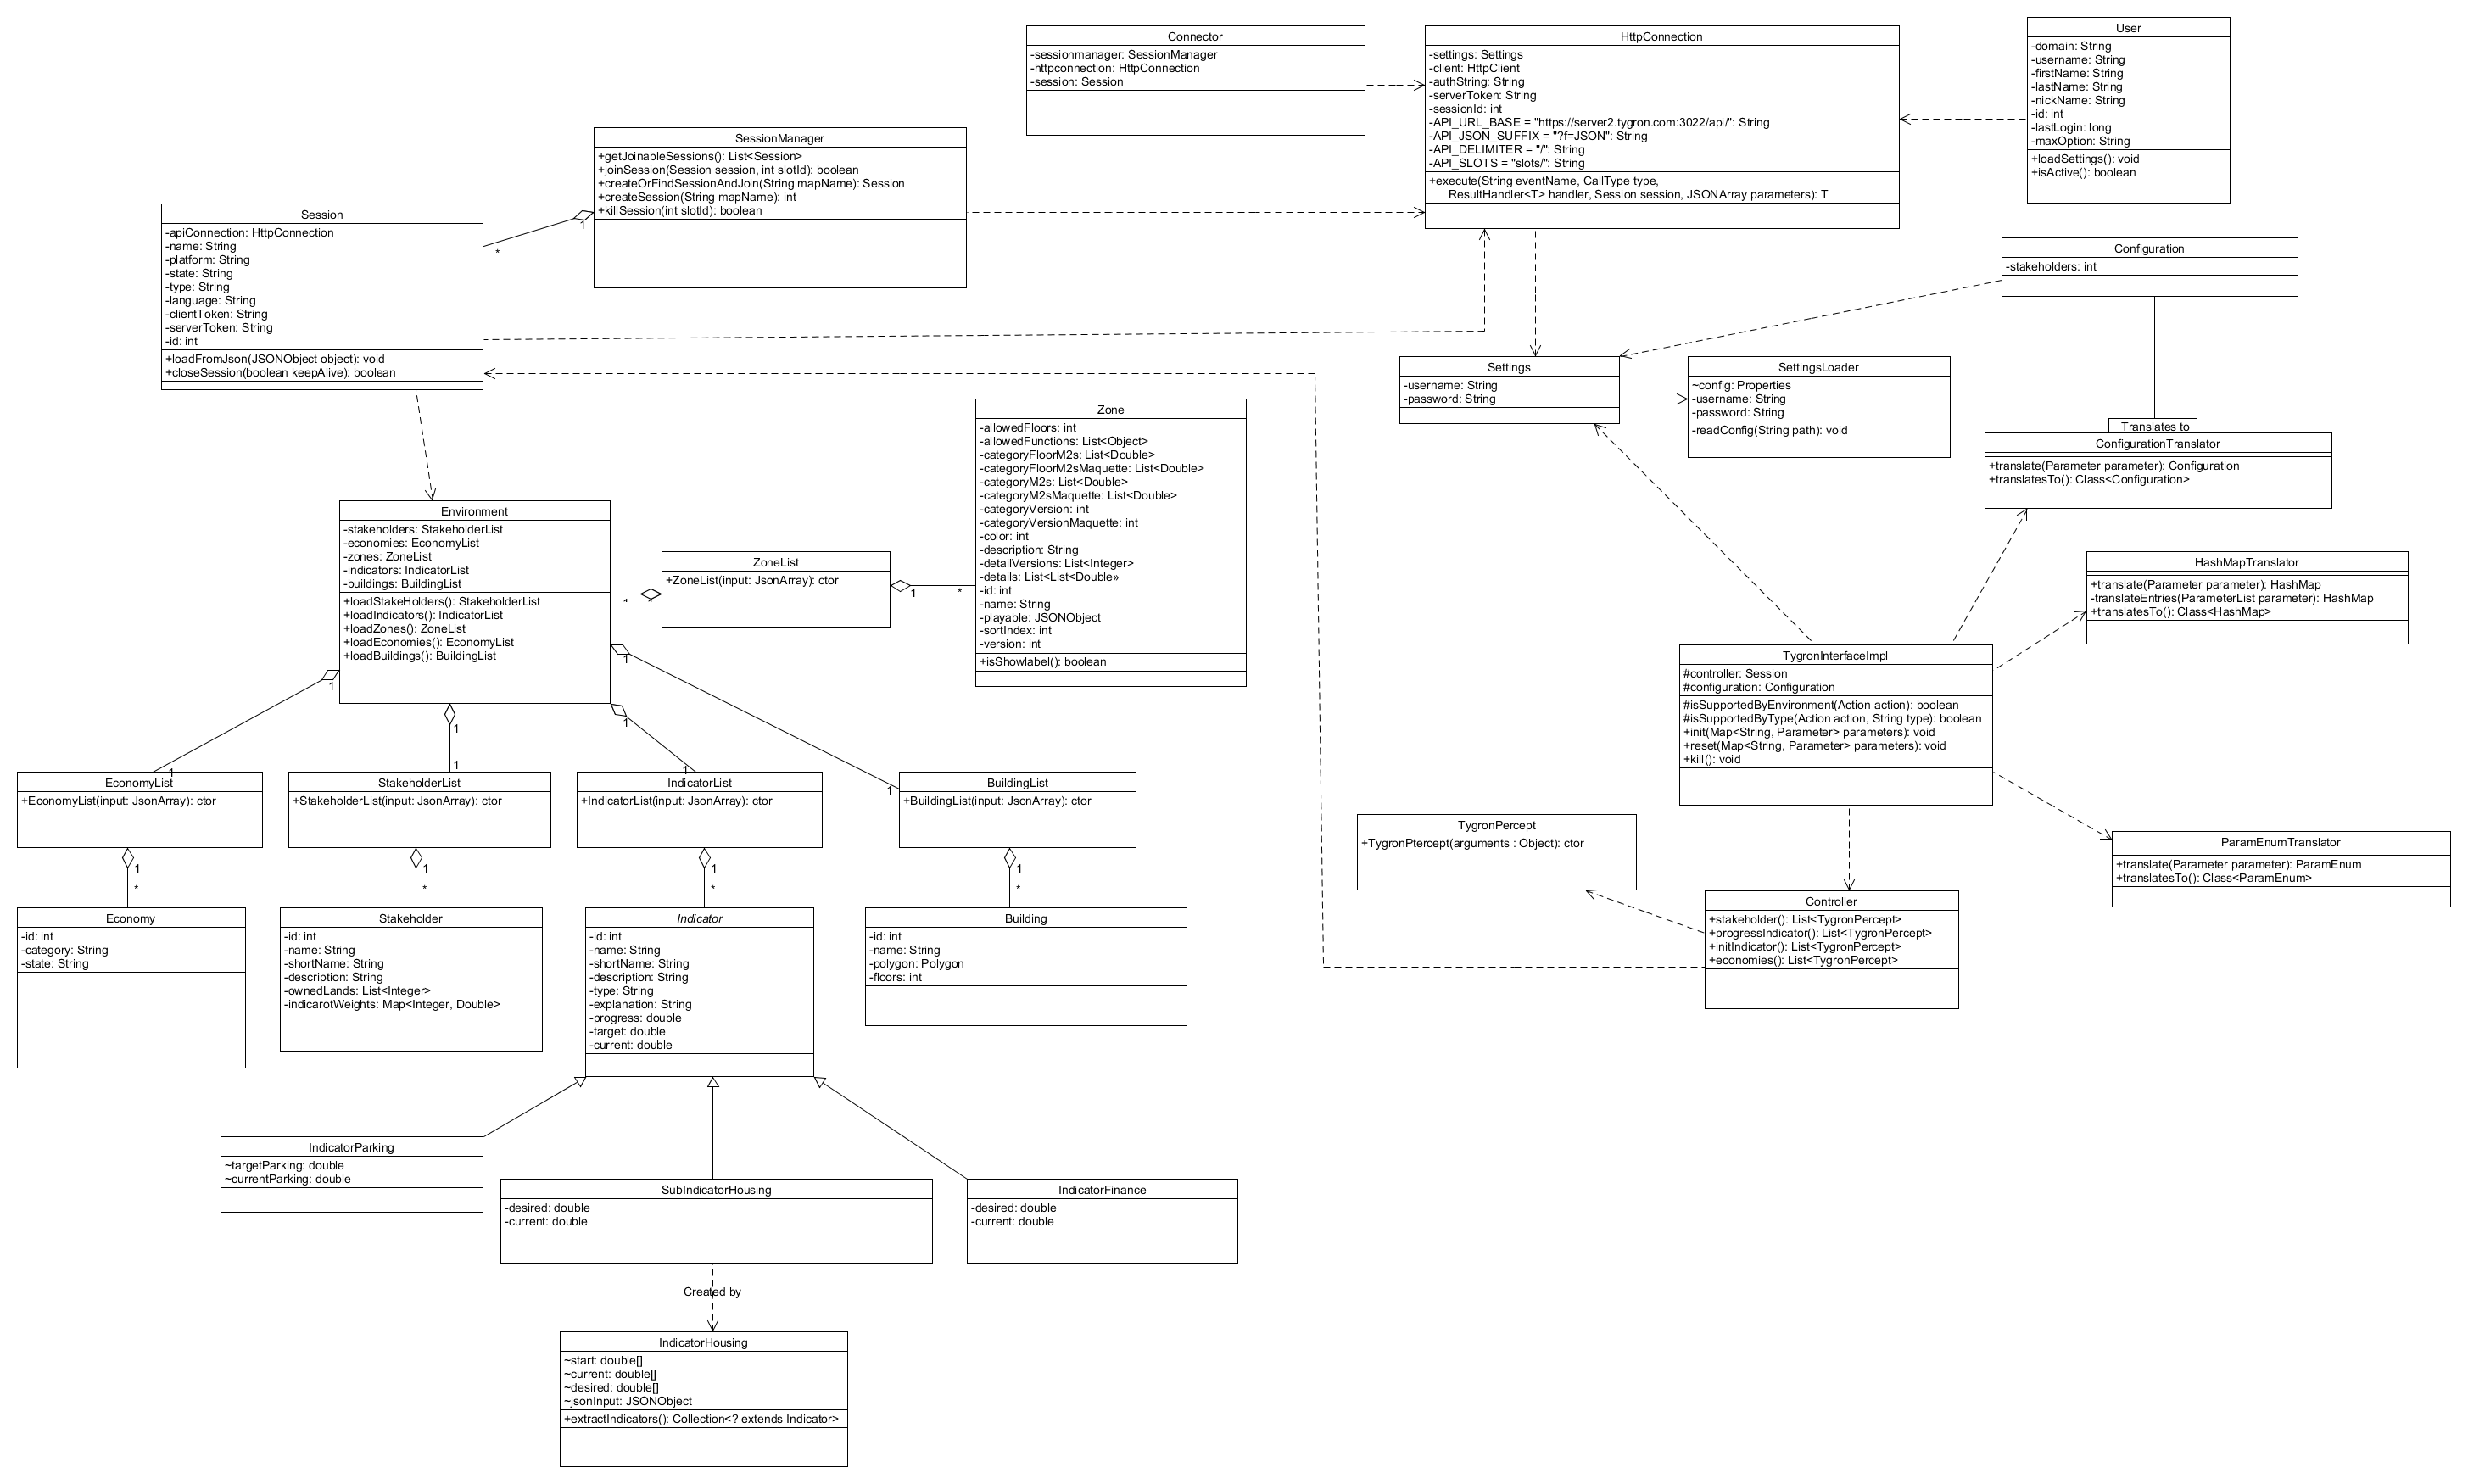
\includegraphics[width=1.0\textwidth]{class diagram.png}
\end{sidewaysfigure}

\clearpage

\section{Software architecture views}
\subsection{Subsystem decomposition}
This part describes our Connector and how it is divided into subsystems.

\begin{figure}[h!]
  \caption{Components diagram}
  \centering
    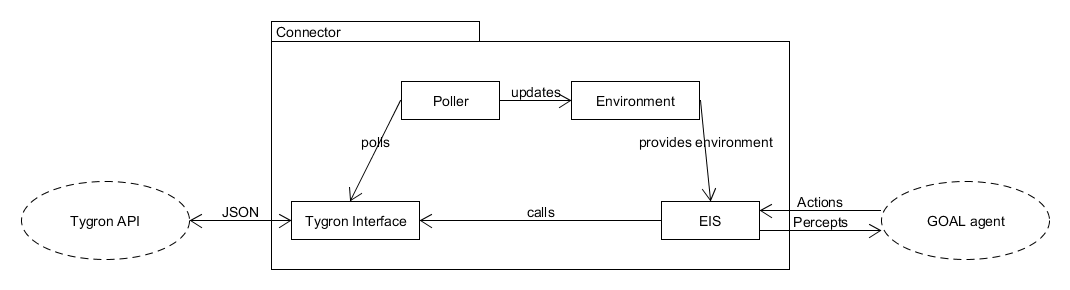
\includegraphics[width=1.0\textwidth]{components diagram.png}
\end{figure}

\subsubsection{Tygron Interface}
The Tygron Interface is a subsystem that will communicate with Tygron’s REST endpoint. This interface’s responsibility is to translate functions to REST requests, and to translate REST responses back to Java objects.

\subsubsection{Environment}
The Environment is a buffer between the EIS and the Tygron Interface. It’s responsibility is to keep a copy of data from the Tygron Interface which can be updated. GOAL agents will be able to access this data via the EIS. The Environment is necessary because otherwise the GOAL agent will be have to wait for the duration of the API request.

\subsubsection{EIS}
We will also develop an interface according to the Environment Interface Standard. This interface is what provides GOAL agents with percepts which will provide GOAL agents with the required information to perform and exposes functions that the agent can call.

\subsubsection{Poller}
It’s job is to poll our JSON interface with some interval, and the results of the polling is used to update the Environment. 

\subsection{Hardware/software mapping}
Our software will communicate over the internet with Tygron’s server. This communication will be layered on HTTP, using the REST protocol.

\subsection{Persistent data management}
Our connector does not have the responsibility of storing persistent data, so it does not have external files or databases.

\subsection{Concurrency}
Our Environment is a shared resource. It is updated by one subsystem and read by another, therefore we are not concerned about deadlocks.

\clearpage
\section{Glossary}
\begin{description}
\item[Cache] \hfill \\
A collection of data which duplicates other data
\item[EIS] \hfill \\
Environment Interface Standard, a standard which facilitates connecting agents to environments
\item[GOAL] \hfill \\
Goal based agent programming language, used for programming intelligent agents
\item[JSON] \hfill \\
JavaScript Object Notation, a data representation format
\item[Percept] \hfill \\
A chunk of data that a GOAL agent receives from it’s environment
\item[Polling] \hfill \\
Sampling an external service
\item[REST] \hfill \\
Representational State Transfer, a software architecture which is used for creating web services
\end{description}

\end{document}

